\documentclass[t, aspectratio=169]{beamer}  % [t], [c], или [b] --- вертикальное выравнивание на слайдах (верх, центр, низ)
%\documentclass[handout]{beamer} % Раздаточный материал (на слайдах всё сразу)

\usetheme{Rochester} % Тема оформления

\usecolortheme{default} % Цветовая схема

%%% Работа с русским языком
\usepackage{cmap}					% поиск в PDF
\usepackage{mathtext} 				% русские буквы в формулах
\usepackage[T2A]{fontenc}			% кодировка
\usepackage[utf8]{inputenc}			% кодировка исходного текста
\usepackage[english,russian]{babel}	% локализация и переносы

%% Beamer по-русски
\newtheorem{rtheorem}{Теорема}
\newtheorem{rproof}{Доказательство}
\newtheorem{rexample}{Пример}

%%% Дополнительная работа с математикой
\usepackage{amsmath,amsfonts,amssymb,amsthm,mathtools} % AMS
\usepackage{icomma} % "Умная" запятая: $0,2$ --- число, $0, 2$ --- перечисление

%% Номера формул
%\mathtoolsset{showonlyrefs=true} % Показывать номера только у тех формул, на которые есть \eqref{} в тексте.
%\usepackage{leqno} % Нумерация формул слева

%% Свои команды
\DeclareMathOperator{\sgn}{\mathop{sgn}}

%% Перенос знаков в формулах (по Львовскому)
\newcommand*{\hm}[1]{#1\nobreak\discretionary{}
{\hbox{$\mathsurround=0pt #1$}}{}}

%%% Работа с картинками
\usepackage{graphicx}  % Для вставки рисунков
\graphicspath{{images/}{images2/}}  % папки с картинками
\setlength\fboxsep{3pt} % Отступ рамки \fbox{} от рисунка
\setlength\fboxrule{1pt} % Толщина линий рамки \fbox{}
\usepackage{wrapfig} % Обтекание рисунков текстом

%%% Работа с таблицами
\usepackage{array,tabularx,tabulary,booktabs} % Дополнительная работа с таблицами
\usepackage{longtable}  % Длинные таблицы
\usepackage{multirow} % Слияние строк в таблице

%%% Программирование
\usepackage{etoolbox} % логические операторы

%%% Другие пакеты
\usepackage{lastpage} % Узнать, сколько всего страниц в документе.
\usepackage{soul} % Модификаторы начертания
\usepackage{csquotes} % Еще инструменты для ссылок

\usepackage[style=authoryear,maxcitenames=3,backend=biber,sorting=nty]{biblatex}
\addbibresource{bib.bib}
\AtBeginBibliography{\tiny} %  Сделаем библиографию меньшим шрифтом
\usepackage{multicol} % Несколько колонок

%%% Картинки
\usepackage{tikz} % Работа с графикой
\usepackage{pgfplots}
\usepackage{pgfplotstable}


\title{Исправление опечаток и грамматических ошибок в русскоязычных текстах}
\author{Бунин Дмитрий, группа 792}
\date{Научный руководитель: канд. физ.-мат. наук Сорокин А. А.}

\begin{document}

\frame[plain]{\titlepage}

\section{Введение и обоснование актуальности}
\begin{frame}
	\frametitle{\insertsection}
	Около 8\%  несловарных слов в ГИКРЯ являются результатом опечаток [\textcite{Shavrina2015}]. \\~\\
	Около 15\% всех поисковых запросов к Яндексу содержат по крайней мере одну ошибку [\textcite{Bajtin2008}]. \\~\\
	Наличие опечаток может существенно влиять на качество современных нейросетевых моделей, таких как BERT [\textcite{Kumar2020}]. \\~\\
	Модуль исправления опечаток --- неотъемлемая часть любого современного текстового редактора.
\end{frame}

\section{Постановка задачи}

\subsection{SpellRuEval}
\begin{frame}
	\frametitle{\insertsection}
	\framesubtitle{\insertsubsection}
	
	Взята задача, поставленная участникам соревнования SpellRuEval [\textcite{Sorokin2016a}], проходившего в рамках конференции <<Диалог 2016>>. \\~\\
	
	В состязании предлагалось исправлять опечатки и грамматические ошибки в текстах из социальных медиа. \\~\\
	
	Все исправляемые грамматические ошибки были локальными, т.е. затрагивали в основном одно слово.
\end{frame}

\subsection{Данные}
\subsubsection{Обучающее множество}
\begin{frame}[allowframebreaks]
	\frametitle{\insertsection} 
	\framesubtitle{\insertsubsection, \insertsubsubsection}
	\begin{itemize}
		\item Количество предложений: 2000.
		\item Всего исправлений: 1727.
		\item Количество уникальных исправлений, неизвестных словарю: 68.
		\item Распределение ошибок по выравниваниям:
			\begin{itemize}
				\item один к одному: 80.0\%;
				\item один ко многим: 15.6\%;
				\item многие к одному: 4.1\%;
				\item многие ко многим: 0.2\%.
			\end{itemize}
		\framebreak
		\item Распределение количества ошибок в предложениях:
		\begin{figure}[!h]
			\begin{center}
				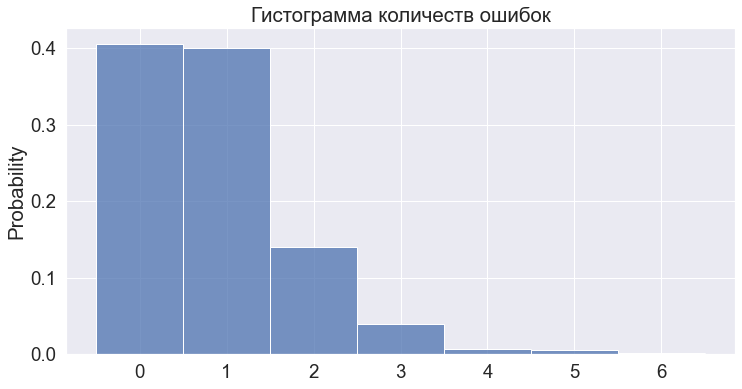
\includegraphics[width=0.8\linewidth]{hist_1}
				\label{ris:hist_1}
			\end{center}
		\end{figure}
	\end{itemize}
\end{frame}

\subsection{Метрики}
\begin{frame}
	\frametitle{\insertsection} 
	\framesubtitle{\insertsubsection}
	Обозначим $S_{cor}$ -- множество корректных исправлений предложений, а $S_{sol}$ -- множество исправлений, выполненных моделью.  Метрики:
	\begin{gather*}
		P = \frac{|S_{sol} \cap S_{cor}|}{|S_{sol}|},
		\\
		R = \frac{|S_{sol} \cap S_{cor}|}{|S_{cor}|},
	\end{gather*}
	Целевая метрика:
	\begin{equation*}
		F_1 = \frac{2 P R}{P + R}.
	\end{equation*}
\end{frame}

\section{Обзор существующих решений}
\subsection{Историческое развитие}
\begin{frame}
	\frametitle{\insertsection} 
	\framesubtitle{\insertsubsection}
	\begin{itemize}
		\item Расстояние Дамерау-Левенштейна.
		\item Модель шумного канала.
		\item Разработка эффективных алгоритмов поиска слов с некоторой ошибкой.
		\item Контекстно-зависимые методы.
	\end{itemize}
\end{frame}

\subsection{Русский язык}
\begin{frame}
	\frametitle{\insertsection} 
	\framesubtitle{\insertsubsection}
	До проведения SpellRuEval почти не было работ для русского языка.  \\~\\
	
	Большая часть из тех, что есть адресованы более конкретным проблемам, например, исправлению поисковых запросов [\textcite{Bajtin2008}], [\textcite{Panina2013}].  \\~\\
	
	Решение победителей SpellRuEval [\textcite{Sorokin2016}] состояло из трех основных этапов:
	\begin{enumerate}
		\item Генерация предложений-гипотез.
		\item Отсечение гипотез при помощи модели ошибок и языковой модели.
		\item Ранжирование оставшихся гипотез логистической регрессией.
	\end{enumerate}
\end{frame}

\section{Описание моделей и методов}

\subsection{Алгоритм}
\begin{frame}
	\frametitle{\insertsection} 
	\framesubtitle{\insertsubsection}
	
	Предварительные действия:
	\begin{enumerate}
		\item Токенизация и нормализация. 
		\item Инициализация <<черного списка>>.
		\item Генерации кандидатов с признаками и объединение токенов в группы. \\~\\
	\end{enumerate} 
	
	Итерации исправления:
	\begin{enumerate}
		\item Поиск лучшей позиции для исправления и проверка критерия останова.
		\item Выбор лучшего исправления .
		\item Внесение позиций без исправлений в <<черный список>>.
	\end{enumerate}
\end{frame}

\subsection{Модуль генерации кандидатов}
\begin{frame}
	\frametitle{\insertsection} 
	\framesubtitle{\insertsubsection}
	Модуль для генерации кандидатов с их признаками. 
	
	Для каждого токена генерируется список кандидатов при помощи моделей:
	\begin{itemize}
		\item \texttt{LevenshteinSearcher}  --- поиск слов на заданном расстоянии Дамерау-Левенштейна. Реализация заимствована из библиотеки DeepPavlov [\textcite{Burtsev2015}].
		\item \texttt{PhoneticSearcher} --- поиск слов с тем же фонетическим кодом. Алгоритм заимствован из решения победителей SpellRuEval.
		\item \texttt{HandcodeSearcher} --- собранная вручную таблица исправлений на корпусе <<Тайга>>. \\~\\
	\end{itemize}
	
	Используется объединение словарей Хагена и wiktionary.  \\~\\
\end{frame}

\subsubsection{Генерация признаков}
\begin{frame}
	\frametitle{\insertsection} 
	\framesubtitle{\insertsubsection, \insertsubsubsection}
	
	Помимо нахождения самих кандидатов для них также вычисляются признаки:
	\begin{itemize}
		\item Признаки позиции.
		\item Признаки источника.
		\item Индикаторы текущего/оригинального кандидатов.
		\item Содержание пробелов/дефисов.
		\item Индикатор словарности.
		\item Индикатор объединения.
	\end{itemize}
\end{frame}

\subsubsection{Объединение токенов}
\begin{frame}
	\frametitle{\insertsection} 
	\framesubtitle{\insertsubsection, \insertsubsubsection}
	В модели генерации кандидатов есть механизм для объединения двух последовательно идущих токенов в один для их совместного рассмотрения. \\~\\
	
	Это нужно для того, чтобы уметь исправлять вставки лишних пробелов: 
	\begin{itemize}
		\item \textit{и так} $\rightarrow$ \textit{итак}, 
		\item \textit{как то} $\rightarrow$ \textit{как-то}. \\~\\
	\end{itemize}
	Алгоритм заключается в последовательном просмотре токенов слева направо и их жадном объединении если получаем словарное слово убрав пробел или заменив его на дефис.
	
\end{frame}

\subsection{Модуль выбора позиции}
\begin{frame}
	\frametitle{\insertsection} 
	\framesubtitle{\insertsubsection}
	Модуль предназначен для выбора позиции исправления и проверки критерия останова.  \\~\\
	
	В его основе лежит использование n-граммных языковых моделей с модифицированным сглаживанием Кнезера-Нея [\textcite{Chen1996}], обученных слева направо и справа налево на корпусе <<Тайга>> [\textcite{Shavrina2017}]. \\~\\
	
	Реализация взята из библиотеки KenLM [\textcite{Heafield2011}, \textcite{Heafield2013}].
\end{frame}

\subsubsection{Алгоритм работы}
\begin{frame}
	\frametitle{\insertsection} 
	\framesubtitle{\insertsubsection, \insertsubsubsection}
	Алгоритм работы:
	\begin{enumerate}
		\item  Для каждой позиции и каждого кандидата находится логарифм вероятности от этих моделей.
		\item Считается агрегирующий показатель --- среднее гармоническое логарифмов вероятностей от левой и правой моделей. Для каждой позиции находится разница показателей между лучшим кандидатом и текущим.
		\item В качестве позиции для исправления позиция берется та, которая
		\begin{itemize}
			\item не находится в <<черном списке>>,
			\item разница показателей в которой максимальна и превышает некий порог.
		\end{itemize}
		\item Вычисленные вероятности и метрика записываются в признаки кандидатов.
	\end{enumerate}
\end{frame}

\subsection{Модуль выбора исправления}
\begin{frame}
	\frametitle{\insertsection} 
	\framesubtitle{\insertsubsection}
	Модуль предназначен для выбора корректного исправления из списка в заданной позиции. \\~\\
	
	Используется модель RuBERT [\textcite{Devlin2019}] [\textcite{Kuratov2019}] или Conversational RuBERT и сгенерированные на предыдущих шагах признаки.
\end{frame}

\subsubsection{Выбор исправления на основе BERT}
\begin{frame}
	\frametitle{\insertsection} 
	\framesubtitle{\insertsubsection, \insertsubsubsection}
	Ранжирование на основе предсказания замаскированных токенов в модели BERT. \\~\\
	
	Алгоритм:
	\begin{enumerate}
		\item Токенизация предложений при помощи WordPiece-токенизатора, использующегося в BERT.
		\item Токенизация кандидатов.
		\item Для каждого подтокена в кандидате измерить логарифм его вероятности, отключив механизм внимания для других подтокенов.
		\item Все полученные логарифмы вероятностей для одного кандидата усреднить.
	\end{enumerate}
\end{frame}

\begin{frame}
	\frametitle{\insertsection} 
	\framesubtitle{\insertsubsection, \insertsubsubsection}
	\begin{figure}[!h]
		\begin{center}
			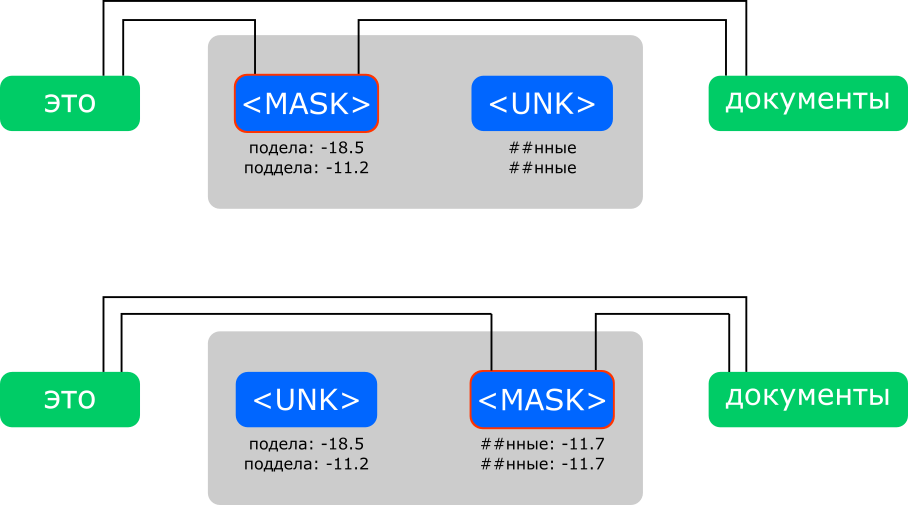
\includegraphics[width=0.7\linewidth]{bert_scoring}
			\caption{Иллюстрация работы ранжирования при помощи BERT.}
			\label{ris:bert_scoring}
		\end{center}
	\end{figure}
\end{frame}

\subsubsection{Выбор исправления на основе множества признаков}
\begin{frame}
	\frametitle{\insertsection} 
	\framesubtitle{\insertsubsection, \insertsubsubsection}
		Было выяснено, что ранжирование только при помощи BERT имеет низкое качество. \\~\\
		
		Протестировав модель на обучающем множестве, удалось собрать выборку, содержащую данные, попадающие в модуль выбора исправления. 
		
		Признаки:
		\begin{itemize}
			\item признаки из модуля генерации кандидатов,
			\item признаки из модуля выбора позиции,
			\item признаки после ранжирования BERT. \\~\\
		\end{itemize}
		
		В качестве моделей над признаками были испытаны ranking SVM [\textcite{Joachims2002}], CatBoost [\textcite{Dorogush2018}].

\end{frame}

\section{Результаты}
\subsection{Сравнение с другими моделями}
\begin{frame}
	\frametitle{\insertsection} 
	\framesubtitle{\insertsubsection}
		\begin{table}
		\begin{center}
			\small
			\begin{tabular}{|c|c|c|c|}
				\hline
				\textbf{Модель} & \textbf{Точность}  & \textbf{Полнота} & $\boldsymbol{F_1}$  \\
				\hline
				Яндекс.Спеллер & 83.09  & 59.86 & 69.59  \\
				JamSpell & 44.57 & 35.69 & 39.64 \\
				SpellRuEval Baseline & 55.91 & 46.41 & 50.72  \\
				SpellRuEval Winner & 81.98 & 69.25 & 75.07  \\
				Только BERT & 48.76 & 57.89 &  52.94 \\
				Лучшая модель & \textbf{87.70} & \textbf{73.23} & \textbf{79.81} \\
				Быстрая модель & 86.04 & 70.80 & 77.68 \\
				\hline
			\end{tabular}
		\end{center}
		\caption{Сравнение результатов различных моделей.}
	\end{table}
\end{frame}

\subsection{Потребление ресурсов}
\begin{frame}
	\frametitle{\insertsection} 
	\framesubtitle{\insertsubsection}
	\begin{itemize}
		\item Скорость лучшей модель: $\approx$ 0.6 предл./с. 
		\item Скорость быстрой модели $\approx$ 4.8 предл./с.
		\item Расход памяти: $\approx$ 7.5ГБ. \\~\\
	\end{itemize}

	Процессор: Intel Core i5-3210M (2 ядра, 4 потока, 2.5ГГц). \\~\\
	
	Такой большой расход памяти вызван хранением словаря в виде префиксного бора и может быть уменьшен в более качественной реализации.
\end{frame}

\section{Заключение}
\begin{frame}
	\frametitle{\insertsection} 
	\vspace{5em}
	\begin{center}
		\huge Спасибо за внимание!
	\end{center}
	\vspace{5em}
	Исходники доступны по ссылке: \url{https://github.com/Mr-Geekman/bd-research}.
\end{frame}

\section{Ответы на вопросы}
\subsection{Примеры работы модели}
\begin{frame}
	\frametitle{\insertsection} 
	\framesubtitle{\insertsubsection}
	\begin{enumerate}
		\item 
		здесь есть только один {\color{red} по настоящему} напряженный момент все остальные {\color{red} давольно} гладкие
		
		здесь есть только один {\color{green} по-настоящему} напряженный момент все остальные {\color{green} довольно} гладкие
		\item 
		да я {\color{red} ваще} за образ жизни а ладах с природой
		
		да я {\color{green} вообще} за образ жизни а ладах с природой
		\item 
		он {\color{red} на столько} крут что я готова {\color{red} приклонятся} перед ним
		
		он {\color{green} настолько} крут что я готова {\color{red} приклонятся} перед ним
		\item 
		{\color{red} остаеться} только кричать его имя в {\color{red} без результат ных} поисках его в этой пустоте
		
		{\color{green} остается} только кричать его имя в {\color{red} без результатных} поисках его в этой пустоте

	\end{enumerate}
\end{frame}

\subsection{Применение модели}
\begin{frame}
	\frametitle{\insertsection} 
	\framesubtitle{\insertsubsection}
	\begin{enumerate}
		\item Создание веб-сервиса по аналогии с Яндекс.Спеллером.
		\item Предварительная обработка текста перед применением методов, чувствительных к опечаткам.
	\end{enumerate}
\end{frame}

\section{Литература}
\begin{frame}[allowframebreaks]{reference}
	\frametitle{\insertsection} 
	\printbibliography
\end{frame}

\end{document}